\documentclass[aspectratio=169]{beamer}

\mode<presentation> {
	\usetheme{Boadilla}
	\setbeamertemplate{headline} % this is the line/code you need to add to get rid of header
}

\setbeamercolor{itemize item}{fg=black}
\setbeamercolor{itemize subitem}{fg=black}
\setbeamercolor{alerted text}{fg=black}
\setbeamertemplate{itemize items}{\textbullet}% отключает кошмарные синие треугольники
\setbeamerfont*{itemize/enumerate subbody}{parent=itemize/enumerate body}
\setbeamerfont*{itemize/enumerate subsubbody}{parent=itemize/enumerate subbody}
\setbeamerfont{alerted text}{series=\bfseries}
% ---------------------------------------------------------------- %
\usepackage{xltxtra}
\usepackage[main=ukrainian,english]{babel}

\setmainfont{Arial}
\setromanfont{Times New Roman}
\setsansfont{Arial}
\setmonofont{Courier New}

\usepackage{indentfirst}
\usepackage{fontspec}

\usepackage{graphicx}
\usepackage{caption}
% для часткових похідних
\usepackage{physics}
\usepackage{mathtools}
\usepackage{mathrsfs, amsmath}
%для картинок
\usepackage{graphicx}
\usepackage{caption}
\usepackage{xcolor}
% для часткових похідних
\usepackage{physics}
\usepackage{amssymb}

\newcommand{\ith}{^{(i)}}
\newcommand{\tran}{^{T}}
% ---------------------------------------------------------------- %
\title{Аналіз атак на лінійні методи машинного навчання}

\author[Середович В.В]{Середович В.В \\ Науковий керівник: Музичук Ю.А.}
\institute{ЛЬВІВСЬКИЙ НАЦІОНАЛЬНИЙ УНІВЕРСИТЕТ ІМЕНІ ІВАНА ФРАНКА \par
Факультет прикладної математики та інформатики \\ Кафедра обчислювальної математики}


\date{\today}

\begin{document}
	% ---------------------------------------------------------------- %
	\begin{frame}
		\titlepage
	\end{frame}
	% ---------------------------------------------------------------- %
	
	\setbeamertemplate{section in toc}{\inserttocsection}
	\begin{frame}
		\tableofcontents
	\end{frame}

	
	% ---------------------------------------------------------------- %
	\section{Постановка задачі}
	\subsection{Етапи роботи}

	\begin{frame}{Постановка задачі}
		\textbf{Змагальний приклад} \\
		Нехай існує класифікатор $f(x):x\rightarrow y$, де  $x \in X, y \in Y$, який передбачає значення $y$ для вхідного $x$. Метою змагального прикладу є знайти такий $x^{*}$, який знаходиться в околі $x$, але хибно визначається класифікатором. Зазвичай максимальний рівень шуму в змагальному прикладі може бути не більше за певну $L_p$ норму $ \| x^{*} - x \|_p < \varepsilon $, де $p=1,2,\infty $. В межах даної роботи для визначення рівня пертурбації буде використовуватись саме $L_{\infty}$ норма.
		\newline
		\newline
		\textbf{Етапи роботи}
		\begin{itemize}
			\item Реалізувати лінійну модель машинного навчання
			\item Розглянути різні методи генерування змагальних прикладів
			\item Застосувати атаки на створену модель та проаналізувати їх ефективність
			\item Розглянути можливі методи захисту від атак
		\end{itemize}
	\end{frame}

	% ---------------------------------------------------------------- %

	\subsection{Модель}
	\begin{frame}{Модель}
		В ролі лінійного методу машинного навчання використовувався алгоритм мультикласової логістичної регресії. \\
		\textbf{Активаційна функція softmax}
		\begin{align*}
			softmax(z_i) = \frac{e^{z_i}}{\sum_{k=1}^{C} e_k^z};
		\end{align*}
		\textbf{Вагова функція кросс-ентропії}
		\begin{align*}
			&\xi(Y, X) =\frac{1}{m} \sum_{i=1}^{m}\xi(y\ith, x\ith) = -\frac{1}{m} \sum_{i=1}^{m} \sum_{j=1}^{C} y_{j}\ith \log (\hat{y}_j\ith) = J(\omega, b)
		\end{align*}
		Для того щоб мінімізувати вагову функцію скористаємость алгоритмом градієнтного спуску.
	\end{frame}
	%% 
	% ---------------------------------------------------------------- %
	\section{Методи атак}
	\subsection{FGSM}
	\begin{frame}{FGSM}
		Ідея Fast Gradient Sign Method методу полягає в тому, щоб знайти такий змагальний приклад $x^{*}$ який максимізує функцію втрати $J(x^{*}, y)$ до певного $L_{\infty}$ обмеження. Цього можна досягти один раз використавши зворотне поширення:
		\begin{equation}
		X^{*} = X + \varepsilon \cdot sign(\Delta_x J(x, y)),
		\end{equation}
		
		
		Для того щоб результат був в $L_{\infty}$ $\varepsilon $ - околі вхідного зображення, будемо використовувати функція образання: $Clip_{\boldsymbol{X}, \varepsilon} \{ \boldsymbol{X}^{*} \}$ - функція яка виконує по-піксельне обрізання зображення $X^{*}$ так,  $\boldsymbol{X}$. 

		\begin{equation}
		Clip_{X, \varepsilon} \{ \boldsymbol{X}^{*} \}(x, y, z) = 
		min\Big\{ 255, \boldsymbol{X}(x, y, z) + \varepsilon, max \{ 0, \boldsymbol{X}(x, y, z) - \varepsilon, \boldsymbol{X}^{*}(x, y, z) \} \Big\}
		\end{equation}
				
		де $\boldsymbol{X}(x, y, z)$ - це значення каналу $z$ зображення $\boldsymbol{X}$ з координатами $(x, y)$.
	\end{frame}
	
	% ---------------------------------------------------------------- %
	
	\subsection{I-FGSM}
	\begin{frame}{I-FGSM}
		Ми застосовуємо звичайний метод декілька разів з певним невеликим кроком α і після кожного кроку використовуємо функцію обрізання, для того щоб переконатись що значення знаходяться в ε-околі оригінального зображення:
		\newline
		
		\centering
		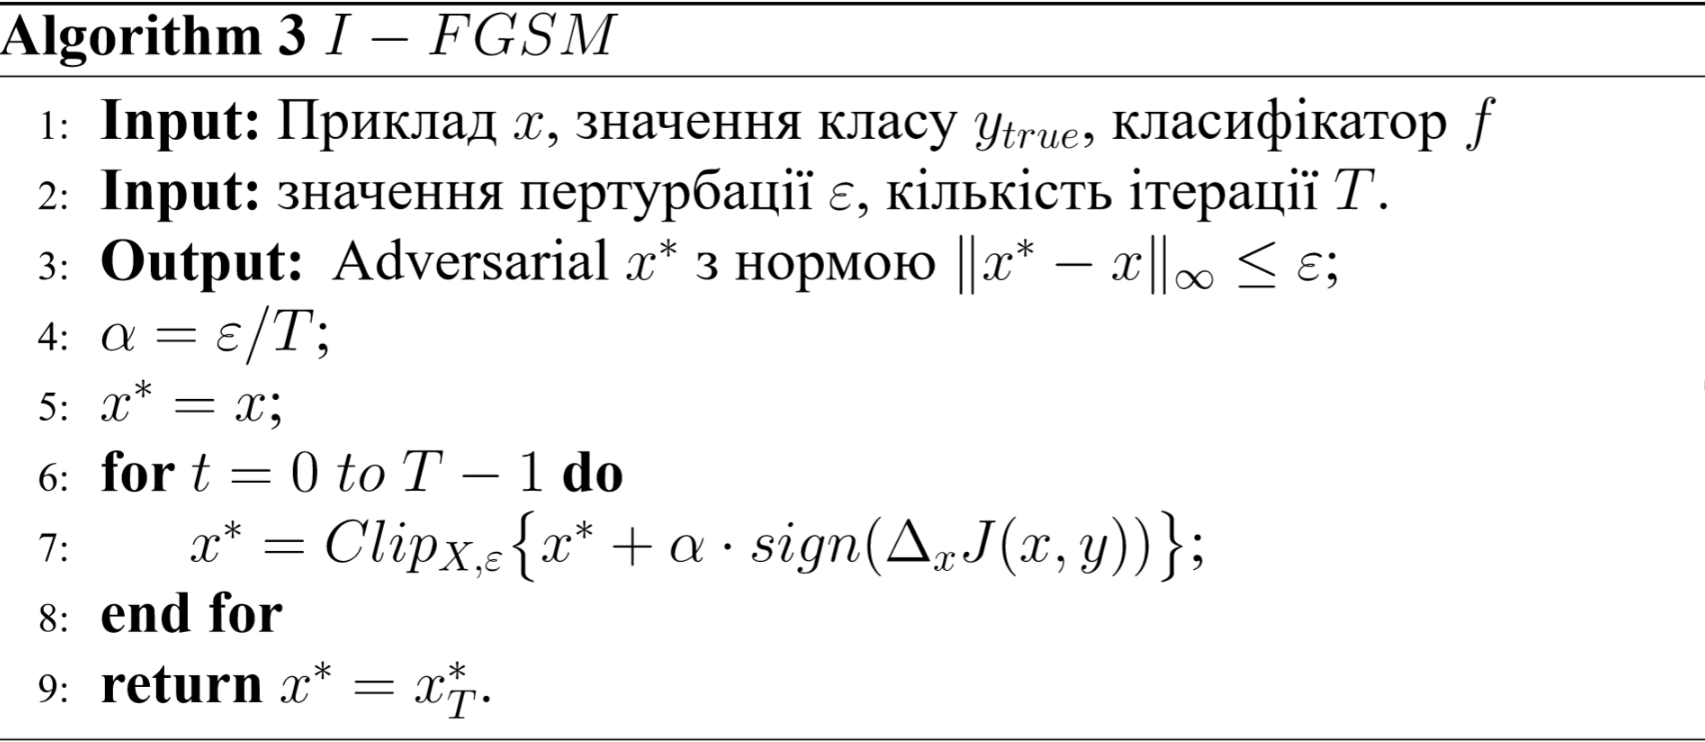
\includegraphics[width=0.9\textwidth]{resources/alg_i-fgsm.png}		
	\end{frame}

	% ---------------------------------------------------------------- %

	\subsection{DeepFool}
	\begin{frame}{DeepFool}
		Для випадку бінарної класифікації легко бачити, що надійність моделі $f$ в точці $ x_{0}$, дорівнює відстані від $x_{0}$ до площини гіперпараметра $\mathscr{F} = \{ x: \omega\tran x + b = 0 \}$, яка розділяє два класи.
		\begin{center}
			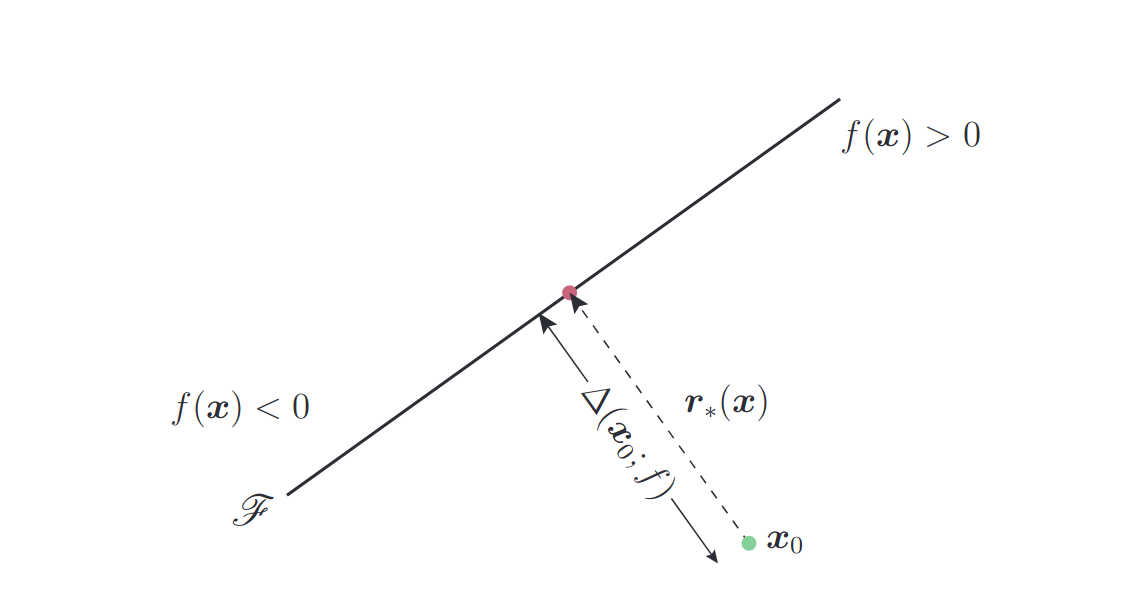
\includegraphics[width=0.8\textwidth]{../CourseWorkLatex/resources/deepfool.jpg}
		\end{center}
	\end{frame}

	% ---------------------------------------------------------------- %
	
	\begin{frame}
		\begin{figure}
			\begin{minipage}[c]{0.67\textwidth}
				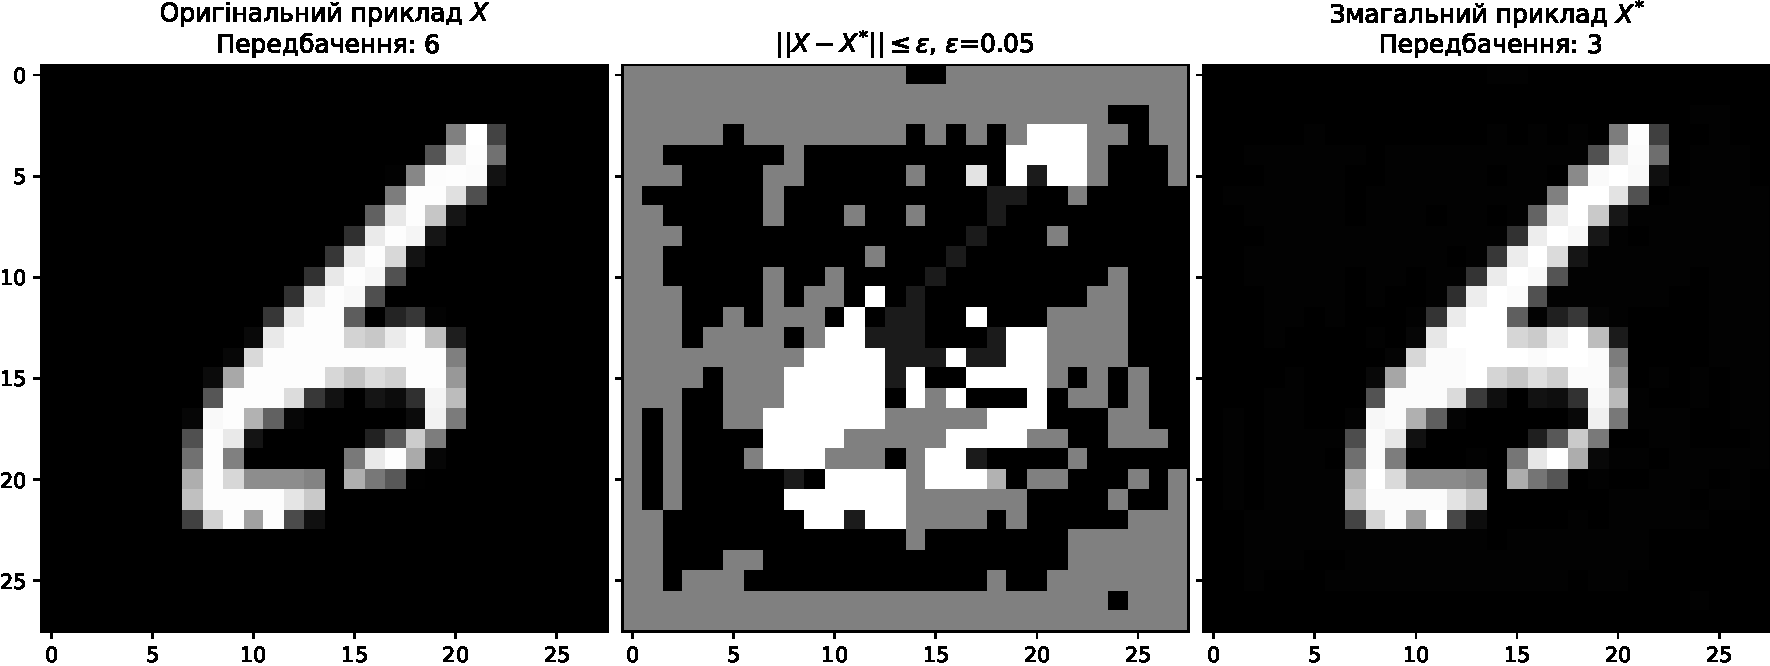
\includegraphics[width=1\textwidth]{../CourseWorkLatex/resources/i-fgsm-example.pdf}
			\end{minipage}\hfill
			\begin{minipage}[c]{0.3\textwidth}
				\caption{
					Результат роботи алгоритму I-FGSM для $\varepsilon = 0.05$
				}
			\end{minipage}
		\end{figure}
		
		\begin{figure}
			\begin{minipage}[c]{0.67\textwidth}
				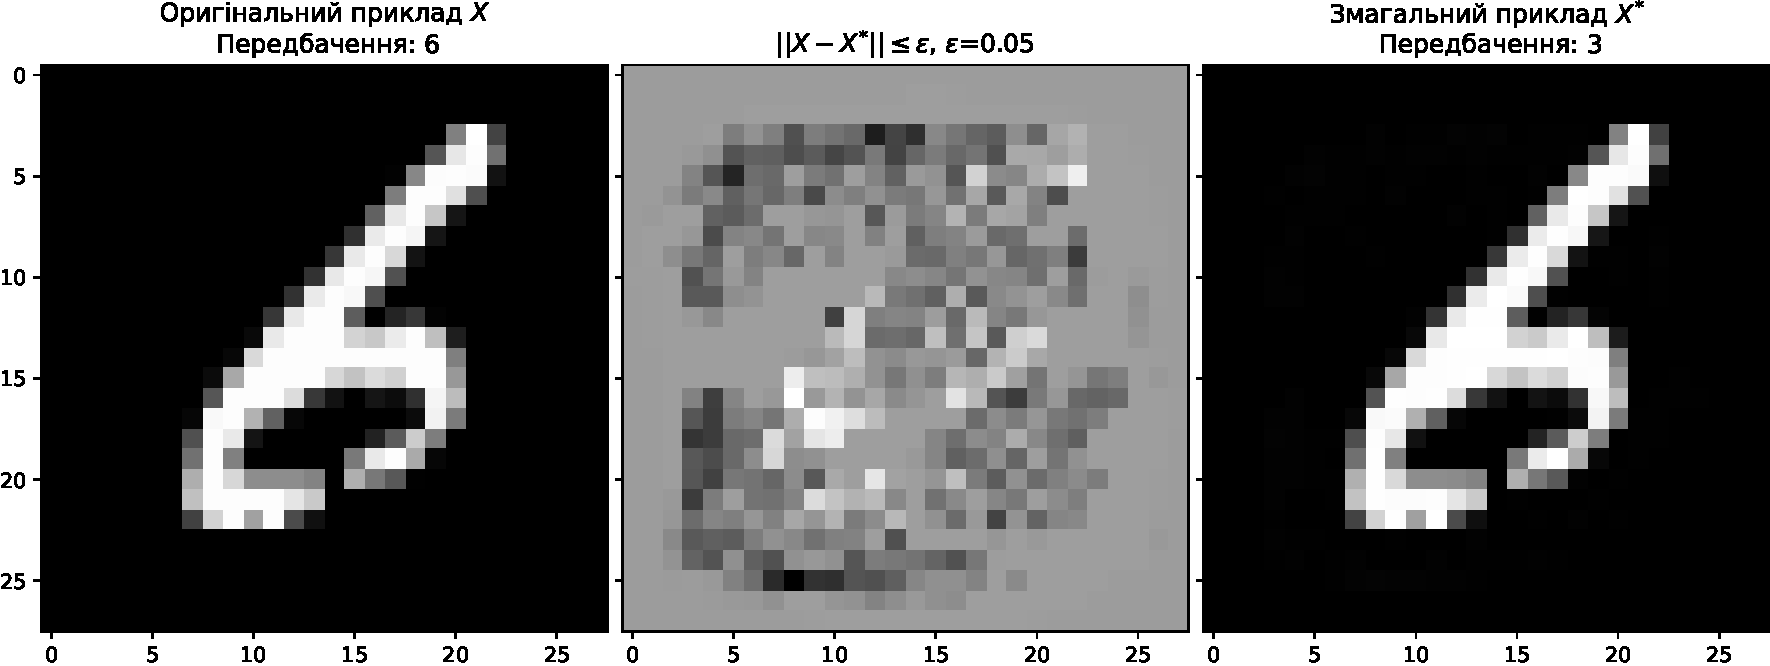
\includegraphics[width=1\textwidth]{../CourseWorkLatex/resources/deepfool-example.pdf}
			\end{minipage}
			\begin{minipage}[c]{0.3\textwidth}
				\caption{
					Результат роботи алгоритму DeepFool для $\varepsilon = 0.05$
				} \hfill
			\end{minipage}
		\end{figure}
	\end{frame}

	% ---------------------------------------------------------------- %
	\section{Методи захисту}
		
	\subsection{Randomization}
	\begin{frame}{Randomization}
		\begin{enumerate}
			\item Оригінальне зображення $x$ розмірами $W \times H \times 1$ замінюють на нове $x'$ з випадково вибраними розмірами $W' \times H' \times 1$.
			\item Другим кроком буде випадкове наповнення деякого простору навколо зображення $x'$ нулями, після чого буде утворене нове зображення $x''$ з розмірами $W'' \times H'' \times 1$.
			\begin{center}
				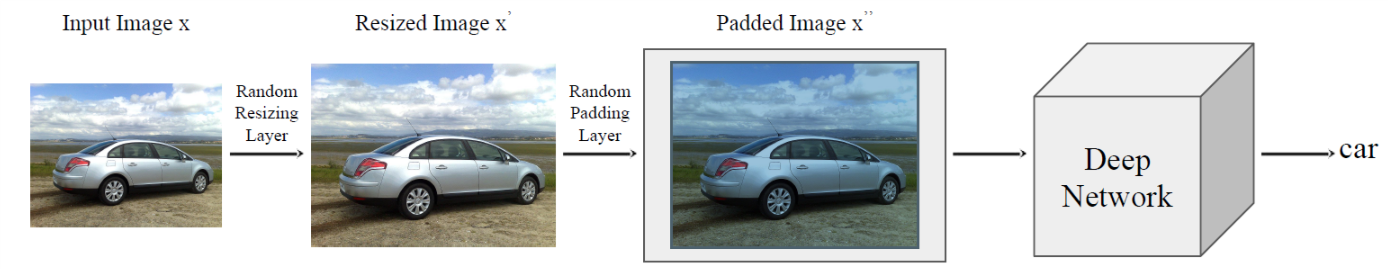
\includegraphics[width=0.95\textwidth]{./resources/randomization.png}
			\end{center}
		\end{enumerate}
	\end{frame}

	\subsection{Pixel Reflection}
	\begin{frame}{Pixel Reflection}
		Ідея методу полягає в тому, щоб випадково вибрати піксель із зображення і потім, так само випадково замінити його на інший піксель в його малому околі.	
		Для того щоб покращити цей алгоритм можна визначити найбільш важливі для класифікації класів місця зображення і уникати їх деформації, знижуючи ймовірність внесення туди змін. Для цього можна скористатись активаційною картою класів моделі. Для випадку нашої моделі вони будуть мати вигляд.
		\begin{center}
			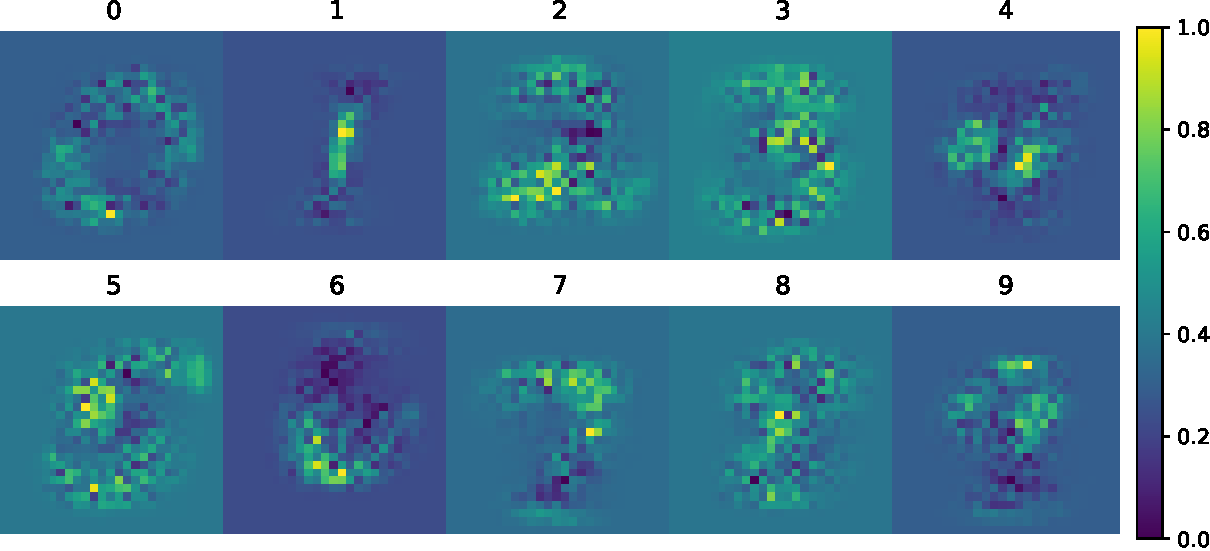
\includegraphics[width=0.7\textwidth]{../CourseWorkLatex/resources/classactivationmap.pdf}
		\end{center}
	\end{frame}

			
	% ---------------------------------------------------------------- %
	\section{Аналіз алгоритмів}
	
	\subsection{Аналіз атак}
	\begin{frame}{Аналіз атак}
		\begin{figure}[!htb]
			\minipage[t]{0.49\textwidth}
			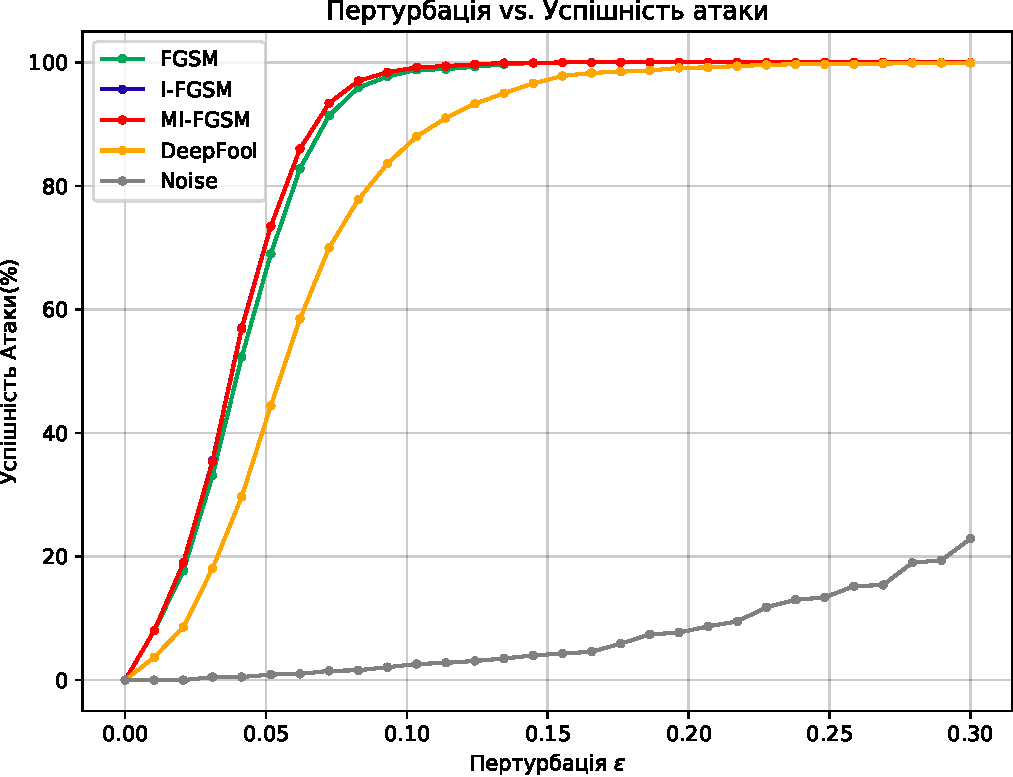
\includegraphics[width=1\textwidth]{../CourseWorkLatex/resources/attacks_bench_8_6.pdf}
			\caption{Графік залежності успішності атаки від величини пертурбації. Нижньою межею буде виступати випадковий шум. }
			\label{fig:attacks_bench}
			\endminipage\hfill
			\minipage[t]{0.49\textwidth}
			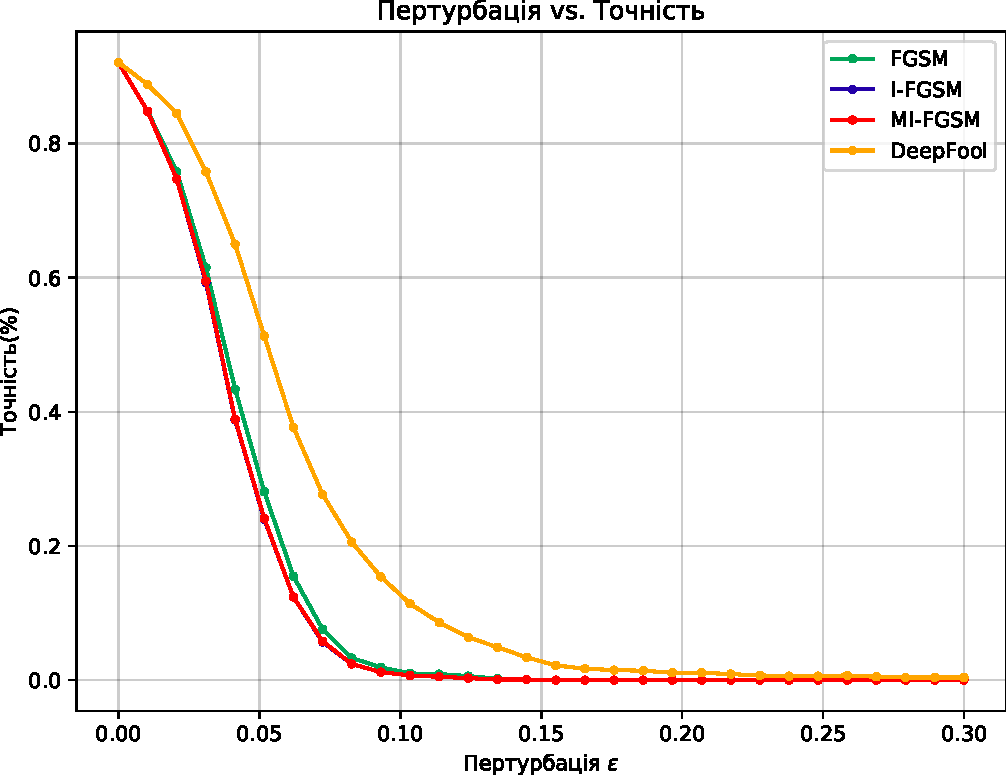
\includegraphics[width=1\textwidth]{../CourseWorkLatex/resources/defenses_bench_8_6.pdf}
			\caption{Графік залежності успішності класифікації моделі від величини пертурбації. Початкова точність моделі \\ $\sim 92\%$}
			\label{fig:defenses_bench}
			\endminipage
		\end{figure}	
	\end{frame}

	\subsection{Аналіз захисту}
	\begin{frame}{Randomization}
	 	Алгоритм випадкової зміни розмірності опинився неефективним для захисту даної 	моделі. Навіть при дуже малих деформаціях зображень, класифікатор починав передбачати їх суттєво гірше і точність моделі знижувалась.

		\begin{figure}[!htb]
			\minipage[t]{0.32\textwidth}
			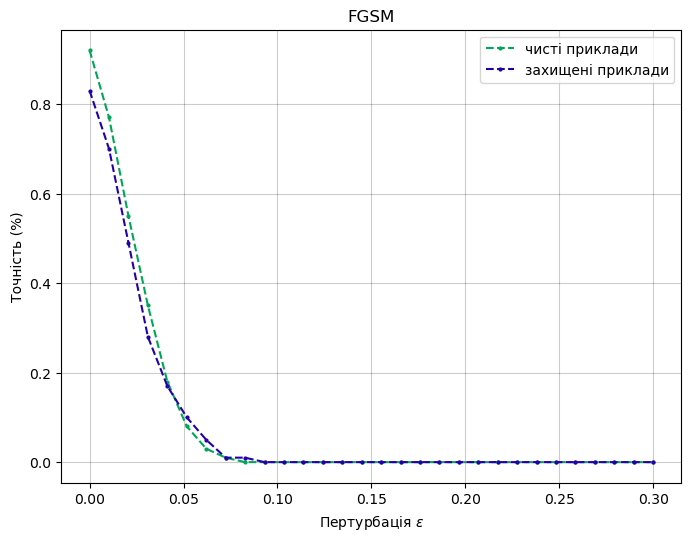
\includegraphics[width=1\textwidth]{../CourseWorkLatex/resources/fgsm_rand_defence.png}
			\endminipage\hfill
			\minipage[t]{0.32\textwidth}
			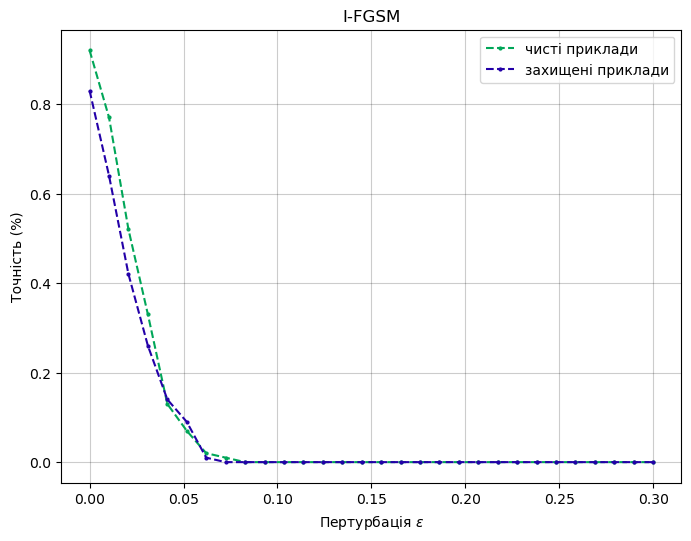
\includegraphics[width=1\textwidth]{../CourseWorkLatex/resources/ifgsm_rand_defence.png}
			\endminipage
			\minipage[t]{0.32\textwidth}
			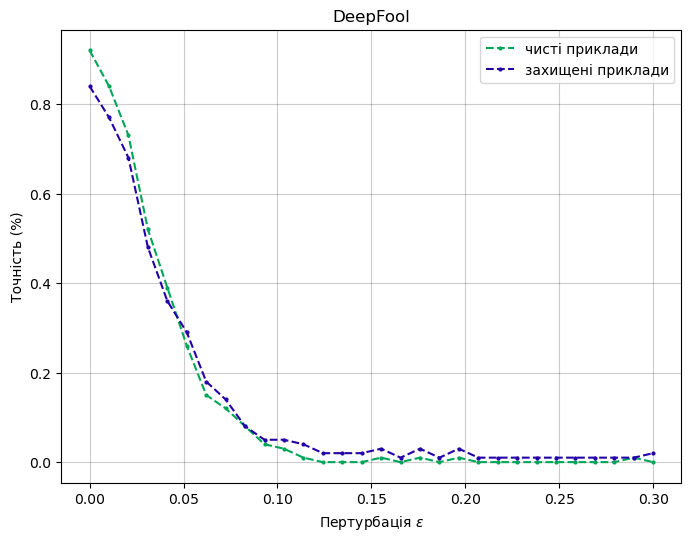
\includegraphics[width=1\textwidth]{../CourseWorkLatex/resources/deepfool_rand_defence.png}
			\endminipage\hfill
			\caption{Randomization}
			\label{fig:randomization}
		\end{figure}
	\end{frame}

	% ---------------------------------------------------------------- %

	\begin{frame}{Pixel Deflection}
		Навіть при відносно великій кількості зсунутих пікселів модель майже не втрачала точність. При оптимальних параметрах деформації вхідного зображення, точність моделі для чистих зображень не падала зовсім, однак успішність проведених атак знижувалась досить слабо, а отже алгоритм не є надійним методом захисту.
		
		\begin{figure}[!htb]
			\minipage[t]{0.32\textwidth}
			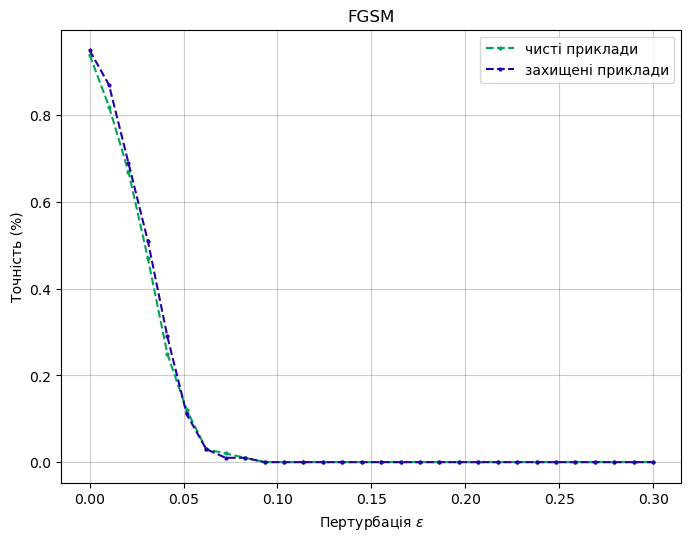
\includegraphics[width=1\textwidth]{../CourseWorkLatex/resources/fgsm_defl_defence.png}
			\endminipage\hfill
			\minipage[t]{0.32\textwidth}
			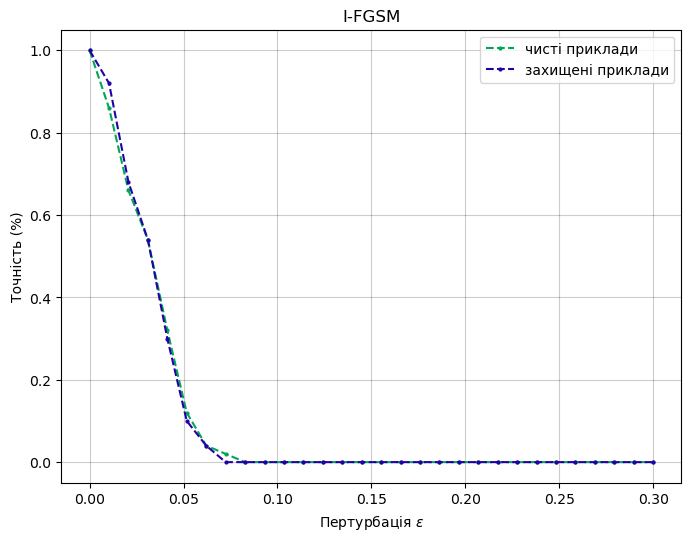
\includegraphics[width=1\textwidth]{../CourseWorkLatex/resources/ifgsm_defl_defence.png}
			\endminipage
			\minipage[t]{0.32\textwidth}
			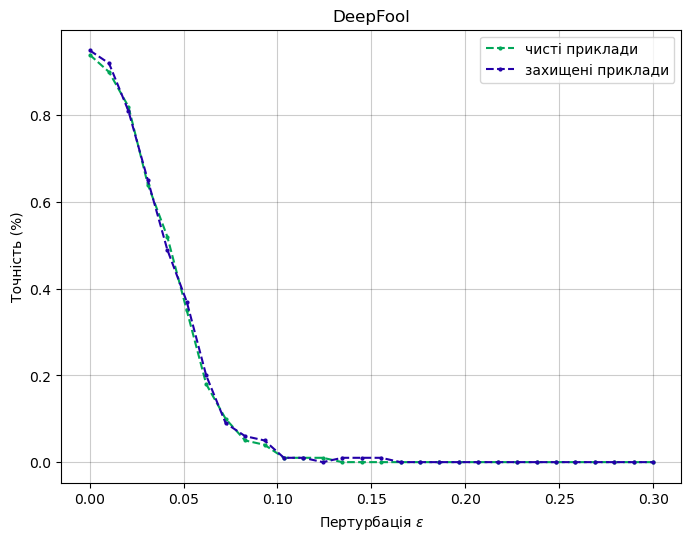
\includegraphics[width=1\textwidth]{../CourseWorkLatex/resources/deepfool_defl_defence.png}
			\endminipage\hfill
			\caption{Pixel Deflection}
			\label{fig:pixeldeflection}
		\end{figure}
	\end{frame}

	% ---------------------------------------------------------------- %
	\section{Висновок}
	\begin{frame}{Висновок}
		
	В межах $L_{\infty}$ норми найефективнішими методами опинились ітераційна модифікація та momentum оптимізація алгоритму FGSM. Також були розглянуті два методи захисту які базуються на ідеї руйнування структури змагальних прикладів через додавання в зображення контрольованого шуму. Методи захисту які базуються на ідеї випадкових деформацій зображень опинились не дуже ефективними у випадку лінійних моделей машинного навчання. 
	
	\end{frame}


\end{document}